
\section{Einzelprozessorsysteme}

\begin{defi}{Überlappte Verarbeitung}
  Ein erstes Ziel der Parallelität war die \emph{überlappte Verarbeitung} von langsamen und schnellen Hardware-Komponenten.
\end{defi}

\begin{example}[Überlappte Verarbeitung]{Direct Memory Access}
  % TODO: https://de.wikipedia.org/wiki/Direct_Memory_Access (Quelle)
  Unter \emph{Direct Memory Access} versteht man, wenn Hardware-Komponenten selbstständig ohne Beteiligung der CPU Daten übertragen können.
  Diese Technik erlaubt anderen Komponenten ohne Umweg über die CPU direkt mit dem Arbeitsspeicher zu kommunizieren.

  Der Vorteil des DMA ist die schnellere Datenübertragung bei gleichzeitiger Entlastung des Prozessors.

  Anders als der Name vermuten lässt, ist die wesentliche Eigenschaft von Direct Memory Access nicht der Speicherzugriff, sondern dass der Datentransfer von einer anderen Komponente und nicht von der CPU selbst initiiert wird. Dabei braucht es zu keinen Speicherzugriffen zu kommen, es sind auch direkte Kommunikationen zwischen Peripheriegeräten möglich

  TODO: Grafik
\end{example}

\begin{defi}{Überlappter I/O}

  TODO: Sinnvolle Definition und Voraussetzungen

  TODO: Grafik
\end{defi}

\subsection{Cache}

\begin{defi}{Cache}
  % TODO: https://de.wikipedia.org/wiki/Cache (Quelle)
  \emph{Cache} bezeichnet einen schnellen Pufferspeicher, der (wiederholte) Zugriffe auf ein langsames Hintergrundmedium oder aufwendige Neuberechnungen zu vermeiden hilft.

  Daten, die bereits einmal geladen oder generiert wurden, verbleiben im Cache, so dass sie bei späterem Bedarf schneller aus diesem abgerufen werden können.

  Auch können Daten, die vermutlich bald benötigt werden, vorab vom Hintergrundmedium abgerufen und vorerst im Cache bereitgestellt werden (\emph{read-ahead}).

  Da es technisch aufwändig und damit meist wirtschaftlich nicht sinnvoll ist, einen Cache zu bauen, der sowohl groß als auch schnell ist, kann man mehrere Caches verwenden -- z. B. einen kleinen schnellen und einen deutlich größeren, jedoch etwas langsameren Cache (der aber immer noch viel schneller ist als der zu cachende Hintergrundspeicher).

  Damit kann man die konkurrierenden Ziele von geringer Zugriffszeit und großem Cacheumfang gemeinsam realisieren.
  Das ist wichtig für die \emph{Hit Rate}.
\end{defi}

\begin{defi}{Cachehierarchie}
  Existieren mehrere Caches, so bilden diese eine \emph{Cachehierarchie}, die Teil der Speicherhierarchie ist.

  Die einzelnen Caches werden nach ihrer Hierarchieebene (engl. \emph{level}) durchnummeriert, also Level-1 bis Level-n oder kurz L1, L2 usw.
  Je niedriger die Nummer, desto näher liegt der Cache an der (schnell) verarbeitenden Komponente;
  die niedrigste Nummer bezeichnet daher den Cache mit der schnellsten Zugriffszeit, dieser wird als erstes durchsucht.

  Enthält der L1-Cache die benötigten Daten nicht, wird der (meist etwas langsamere, aber größere) L2-Cache durchsucht usw.
  Das geschieht solange, bis die Daten entweder in einer Cacheebene gefunden (\emph{Cache Hit}) oder alle Caches ohne Erfolg durchsucht wurden (\emph{Cache Miss}).
  In letzterem Fall muss auf den langsamen Hintergrundspeicher zugegriffen werden.
\end{defi}

\begin{example}[Cachehierarchie]{Harvard-Architektur}
  % TODO: https://en.wikipedia.org/wiki/Cache_hierarchy (Quelle, Grafiken)
\end{example}

\begin{defi}[Cache]{Zugriffszeit}
  Durch die Aufteilung des L1-Cache in Daten- und Instruktions-Cache (Harvard-Architektur) können bei Pipeline-basierten Rechnern gleichzeitig neue Instruktionen zum Füllen der Pipeline geholt werden und bei der Bearbeitung der Operanden die Daten ausgelesen werden.

  Die \emph{Zugriffszeit} $t_Z$ eines Caches kann wie folgt definiert werden:
  \[
    t_Z = t_{C} + (1 - h) \cdot t_{M}
  \]
  Dabei ist $t_C$ die Zugriffszeit des Prozessors für Werte aus dem Cache, $t_M$ die für Daten aus dem Memory und $h$ die Hit-Rate.

  Wenn die Hit-Rate groß sein soll, sind sowohl ein Programm mit hoher räumlicher und zeitlicher Lokalität, sowie ein großer Cache (meist L1, L2 und L3) erforderlich.
\end{defi}

\begin{defi}{Direct Mapped Cache}
  % TODO: https://en.wikipedia.org/wiki/Cache_placement_policies#Direct-mapped_cache (Quelle)
  Bei einem \emph{Direct Mapped Cache} wird der Hauptspeicher in mehreren disjunkte Untermengen organisiert, wobei pro Untermenge genau eine Cache-Zeile definiert ist.

  Platzieren eines Speicherblocks im Cache:
  \begin{itemize}
    \item Bestimmen der Zeilenadresse im Cache, basierend auf Adresse um Hauptspeicher
    \item Speicherblock wird entsprechend im Cache gespeichert, als Tag wird die Hauptspeicheradresse verwendet
    \item vorher gespeicherte Daten werden überschrieben
  \end{itemize}

  Suchen im Cache:
  \begin{itemize}
    \item Bestimmen der Zeilenadresse im Cache, basierend auf Adresse um Hauptspeicher
    \item Tags (Hauptspeicheradressen) werden verglichen
    \item bei gleichen Tags \emph{Cache-Hit}, sonst \emph{Cache-Miss}
    \item bei einem \emph{Cache-Miss} muss der Speicherblock in Cache geladen werden
  \end{itemize}

  Vorteile des Direct Mapped Cache sind, dass nicht alle Adressen im Cache durchsucht werden müssen und das Vorgehen sehr simpel ist.

  Da allerdings pro Untermenge im Hauptspeicher nur eine Zeile im Cache definiert ist, ist die Hit-Rate geringer als bei Alternativen.

  \centering
  % TODO: https://diveintosystems.org/book/C11-MemHierarchy/caching.html (Quelle)
  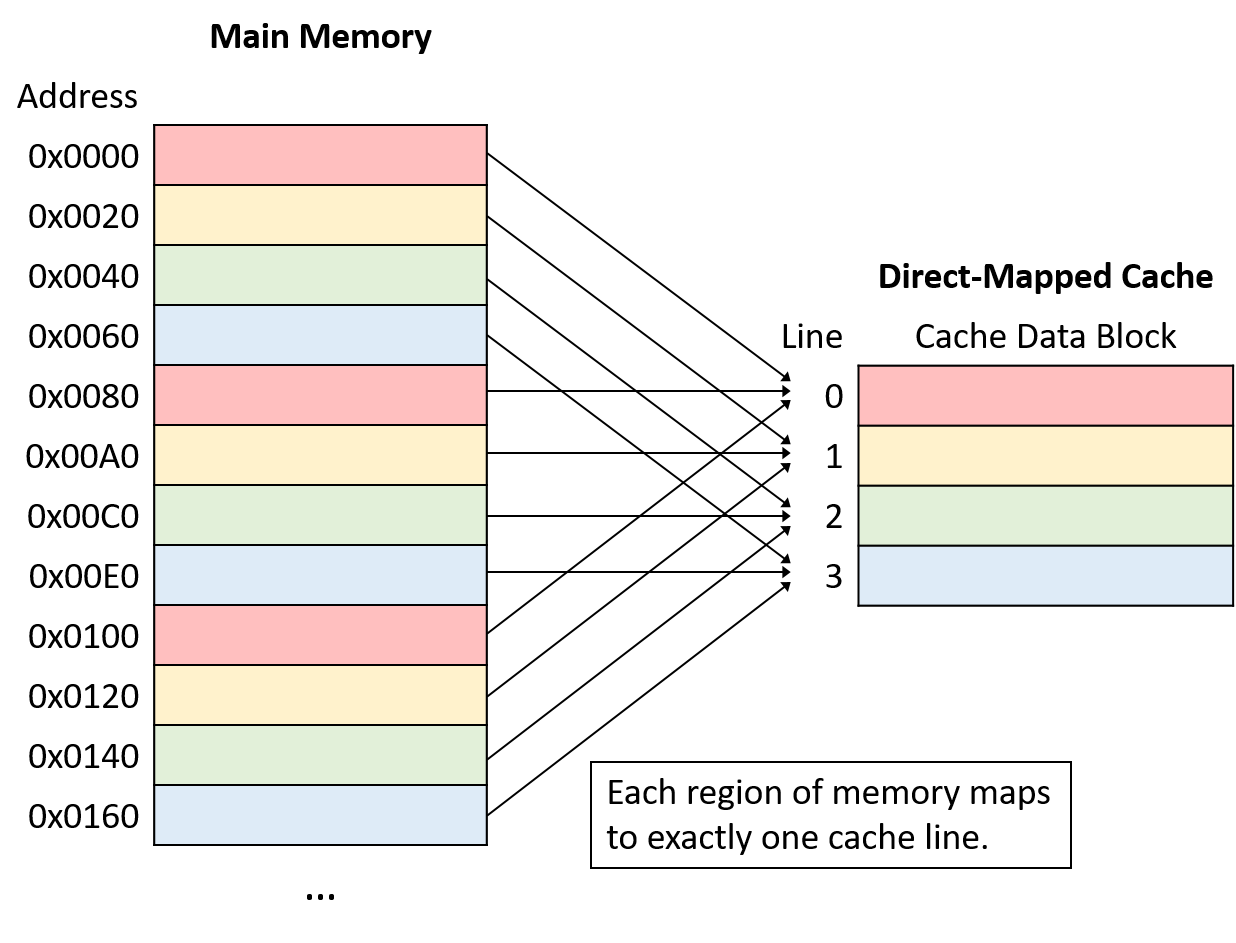
\includegraphics[width=.6\linewidth]{images/direct_mapped_cache.png}
  % 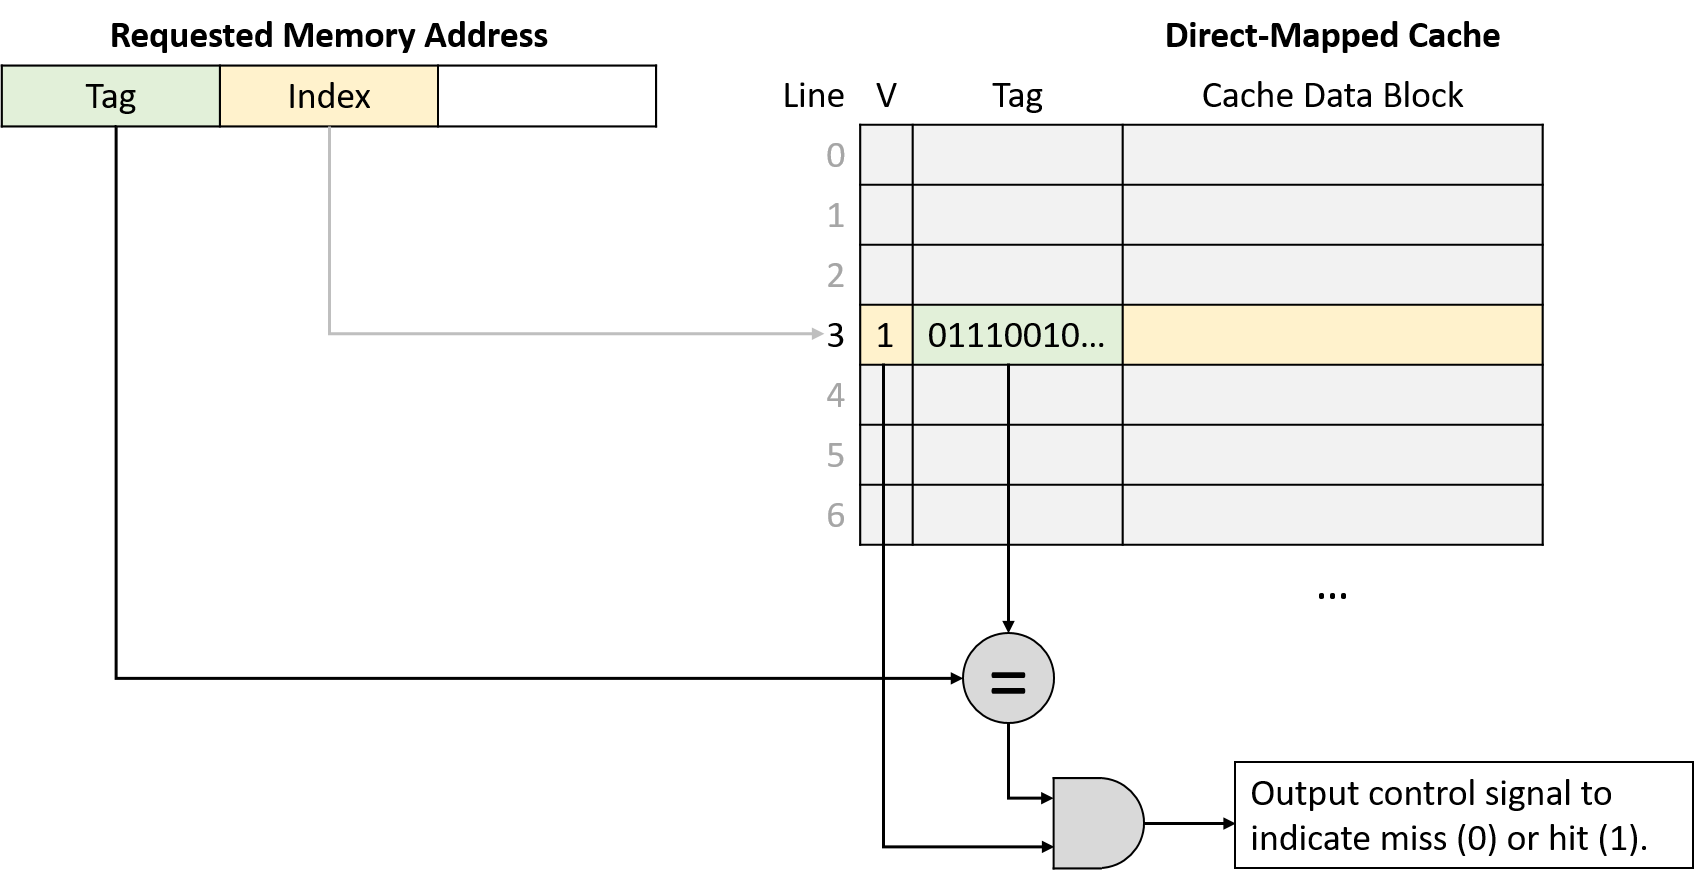
\includegraphics[width=.9\linewidth]{images/direct_mapped_cache_request.png}
\end{defi}

\begin{defi}{N-way Set Associative Cache}


  % TODO: https://diveintosystems.org/book/C11-MemHierarchy/caching.html (Quelle)
  \centering
  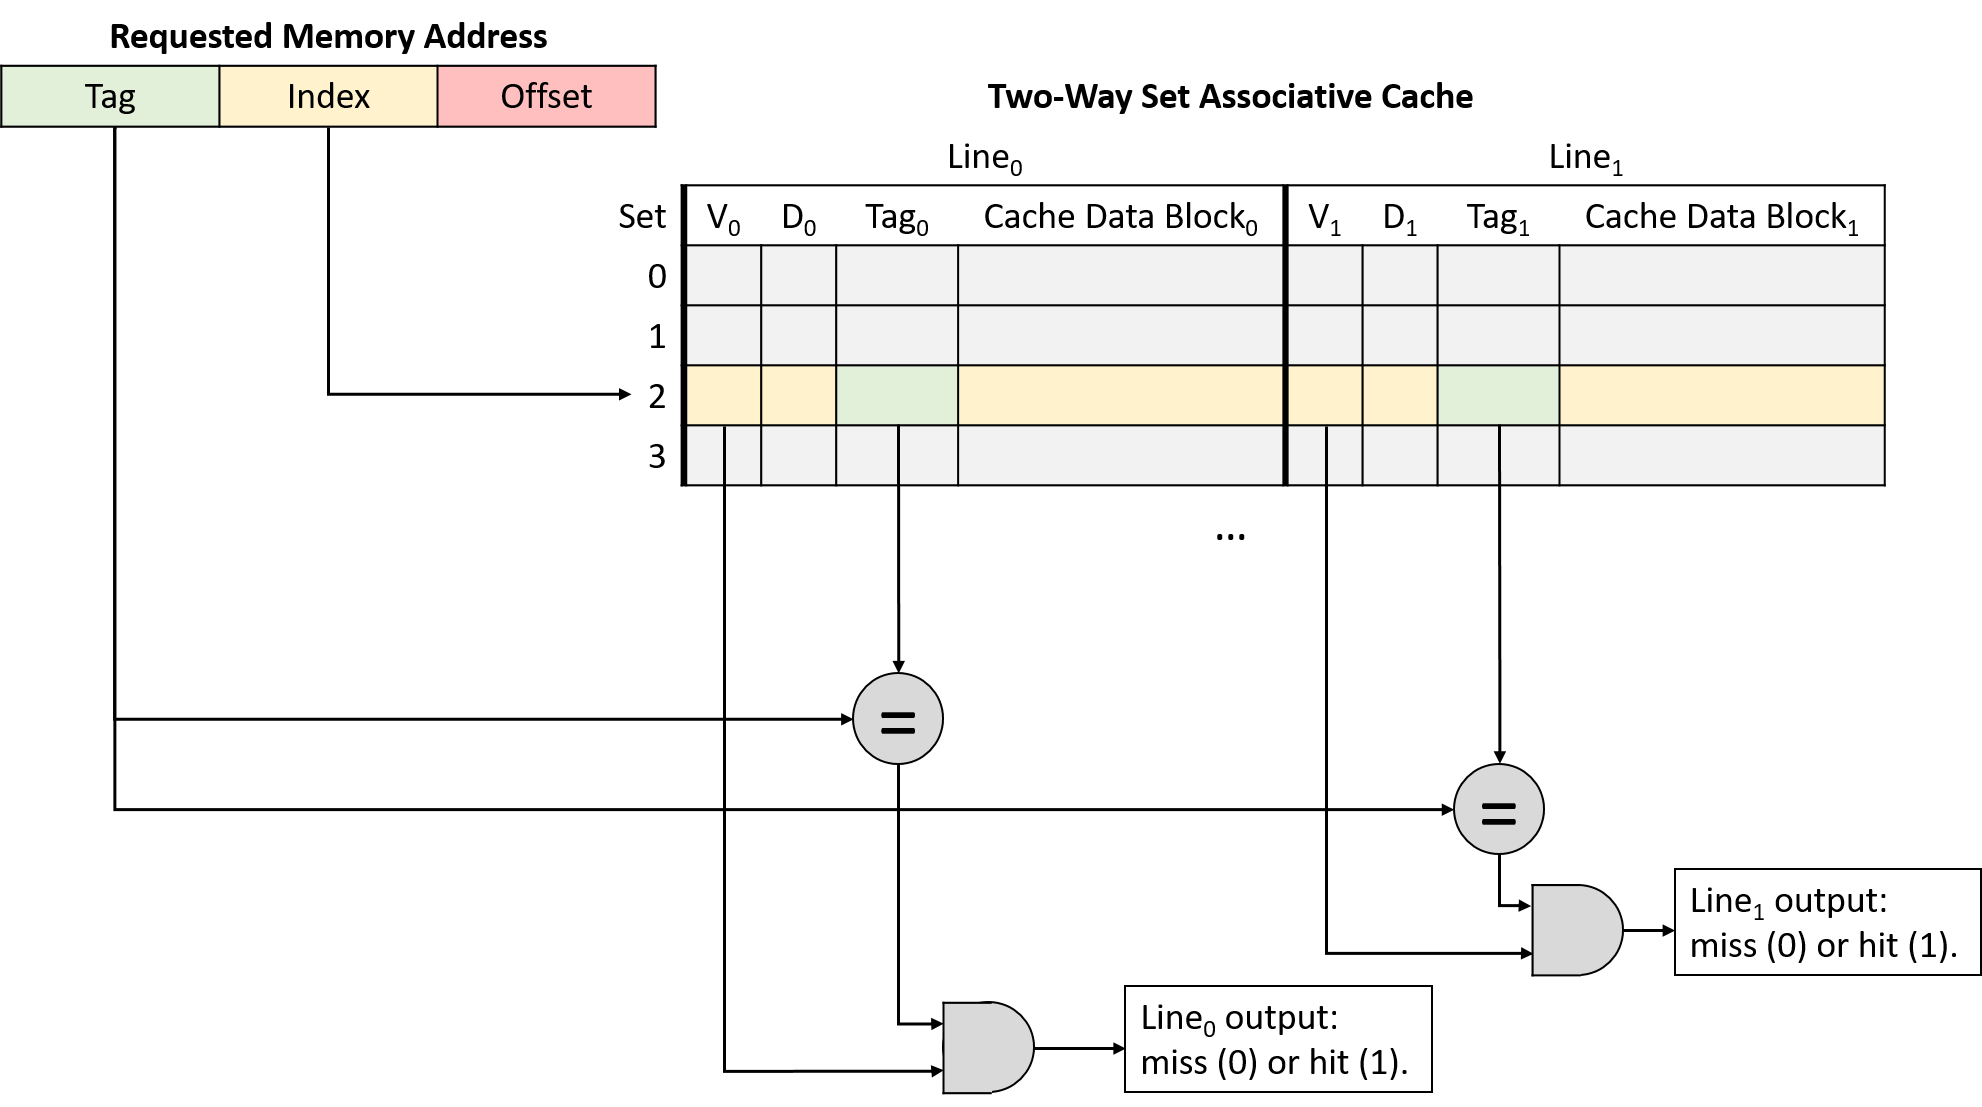
\includegraphics[width=.9\linewidth]{images/2-way_set_associative_cache_request.png}
\end{defi}

\begin{example}[N-way Set Associative Cache]{2-way Set Associative Cache}
\end{example}

\begin{defi}{Fully Associative Cache}

\end{defi}

\begin{defi}{Ersetzungsstrategie}

\end{defi}

\begin{bonus}[Cache]{IBM Power 4}

\end{bonus}

\begin{bonus}[Cache]{Intel Itanium}

\end{bonus}

\begin{defi}{Cache Miss}

\end{defi}

\begin{defi}{Reduzierung der Cache Miss Rate}

\end{defi}

\begin{defi}[Reduzierung der Cache Miss Rate]{Programmierstrategien}

\end{defi}

\begin{defi}{Table-Look-Aside Buffer}

\end{defi}

\subsection{Entwicklungslinien der Prozessoren}

\begin{defi}{CISC}

\end{defi}

\begin{defi}{RISC}

\end{defi}

\begin{defi}{VLIW}

\end{defi}

\begin{defi}{EPIC}

\end{defi}